%------------------------------------------------------------------------------
% CV in Latex
% Author : Charles Rambo
% Based off of: https://github.com/sb2nov/resume and Jake's Resume on Overleaf
% Most recently updated version may be found at https://github.com/fizixmastr 
% License : MIT
%------------------------------------------------------------------------------

\documentclass[A4,11pt]{article}
%\documentclass[letterpaper,11pt]{article} %For use in US
\usepackage{latexsym}
\usepackage[empty]{fullpage}
\usepackage{titlesec}
\usepackage{marvosym}
\usepackage[usenames,dvipsnames]{color}
\usepackage{verbatim}
\usepackage{enumitem}
\usepackage[hidelinks]{hyperref}
\usepackage[english]{babel}
\usepackage{tabularx}
\usepackage{tikz}
\usepackage[super]{nth}
\input{glyphtounicode}

\begin{comment}
I am by no means a professional when it comes to the CV's/resumes, I have
received various trainings on how to write a CV and resume from my high 
school, as well as the Austin College and University of Eastern Finland's
career counseling departments. As I intend to share my CV as a template, I 
feel that it is my responsibility to provide explanations of my work.
\end{comment}


%-----FONT OPTIONS-------------------------------------------------------------
\begin{comment}
The font of the document will impact not just how readable it is, but how it is
perceived. In the "The Craft of Scientific Writing" by Michael Alley, shares a
common fonts for publication as well as their use. I have chosen to use
Palatino for its legibility, some others are given below. There is far too much
about typography to discus here. Note: serif fonts have short projecting
strokes, sans-serif fonts are sans (without) these strokes.
\end{comment}


% serif
 \usepackage{palatino}
% \usepackage{times} %This is the default as well
% \usepackage{charter}

% sans-serif
% \usepackage{helvet}
% \usepackage[sfdefault]{noto-sans}
% \usepackage[default]{sourcesanspro}

%-----PAGE SETUP---------------------------------------------------------------

% Adjust margins
\addtolength{\oddsidemargin}{-1cm}
\addtolength{\evensidemargin}{-1cm}
\addtolength{\textwidth}{2cm}
\addtolength{\topmargin}{-1cm}
\addtolength{\textheight}{2cm}

% Margins for US Letter size
%\addtolength{\oddsidemargin}{-0.5in}
%\addtolength{\evensidemargin}{-0.5in}
%\addtolength{\textwidth}{1in}
%\addtolength{\topmargin}{-.5in}
%\addtolength{\textheight}{1.0in}

\urlstyle{same}

\raggedbottom
\raggedright
\setlength{\tabcolsep}{0cm}

% Sections formatting
\titleformat{\section}{
  \vspace{-4pt}\scshape\raggedright\large
}{}{0em}{}[\color{black}\titlerule \vspace{-5pt}]

% Ensure that .pdf is machine readable/ATS parsable
\pdfgentounicode=1

%-----CUSTOM COMMANDS FOR FORMATTING SECTIONS----------------------------------
\newcommand{\CVItem}[1]{
  \item\small{
    {#1 \vspace{-2pt}}
  }
}

\newcommand{\CVSubheading}[4]{
  \vspace{-2pt}\item
    \begin{tabular*}{0.97\textwidth}[t]{l@{\extracolsep{\fill}}r}
      \textbf{#1} & #2 \\
      \small#3 & \small #4 \\
    \end{tabular*}\vspace{-7pt}
}

\newcommand{\CVSubSubheading}[2]{
    \item
    \begin{tabular*}{0.97\textwidth}{l@{\extracolsep{\fill}}r}
      \text{\small#1} & \text{\small #2} \\
    \end{tabular*}\vspace{-7pt}
}

\newcommand{\CVSubItem}[1]{\CVItem{#1}\vspace{-4pt}}

\renewcommand\labelitemii{$\vcenter{\hbox{\tiny$\bullet$}}$}

\newcommand{\CVSubHeadingListStart}{\begin{itemize}[leftmargin=0.5cm, label={}]}
% \newcommand{\resumeSubHeadingListStart}{\begin{itemize}[leftmargin=0.15in, label={}]} % Uncomment for US
\newcommand{\CVSubHeadingListEnd}{\end{itemize}}
\newcommand{\CVItemListStart}{\begin{itemize}}
\newcommand{\CVItemListEnd}{\end{itemize}\vspace{-5pt}}

%\pagestyle{plain}

%------------------------------------------------------------------------------
% CV STARTS HERE  %
%------------------------------------------------------------------------------
\begin{document}

%-----HEADING------------------------------------------------------------------
\begin{comment}
In Europe it is common to include a picture of ones self in the CV. Select
which heading appropriate for the document you are creating.
\end{comment}

\begin{minipage}[c]{0.05\textwidth}
\-\
\end{minipage}
\begin{minipage}[c]{0.2\textwidth}
\begin{tikzpicture}
    \clip (0,0) circle (1.5cm);
    \node at (0,0) {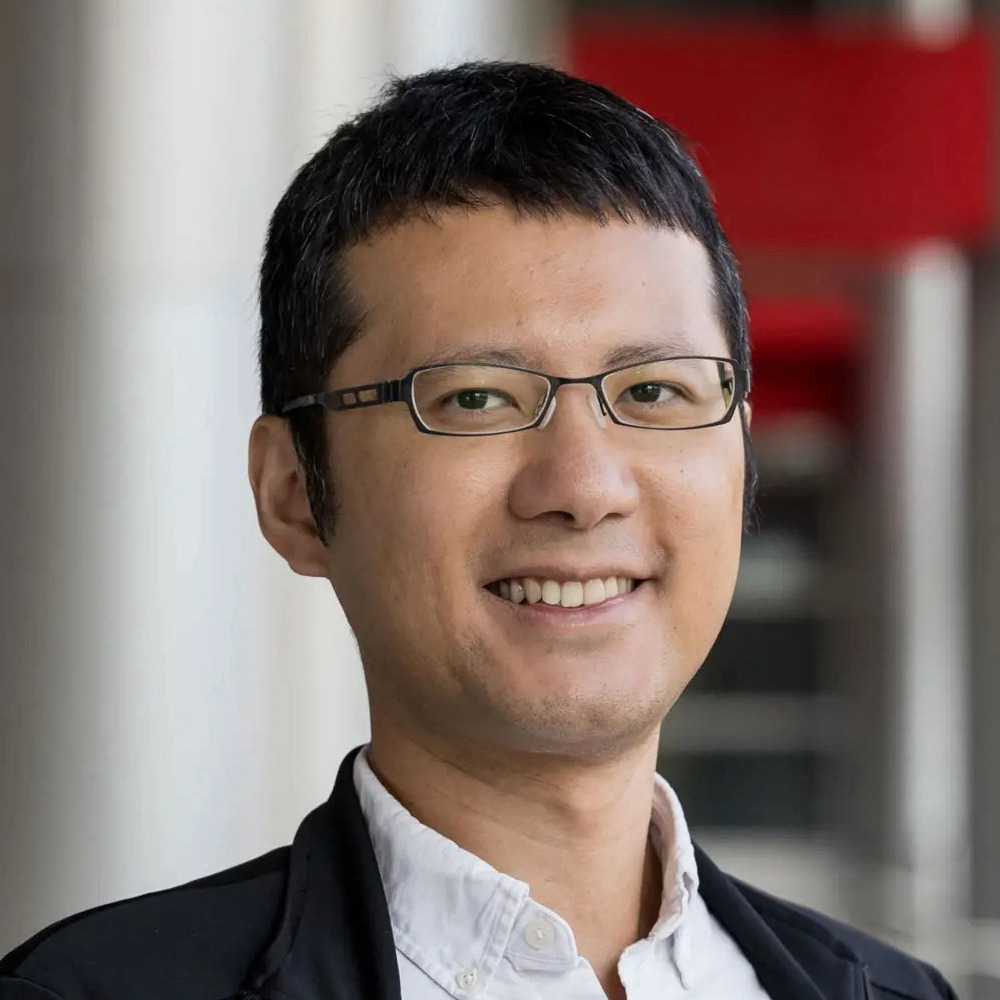
\includegraphics[width = 3cm]{twhuang_uwm.jpg}}; 
    \draw (0,0) circle (1.5cm);
    % if necessary the picture may be moved by changing the at (coordinates)
    % width defines the 'zoom' of the picture
\end{tikzpicture}
\hfill\vline\hfill
\end{minipage}
\begin{minipage}[c]{0.6\textwidth}
    \textbf{\Huge \scshape{ Tsung-Wei (TW) Huang}} \\ \vspace{2pt} 
    % \scshape sets small capital letters, remove if desired
    \small{} \\
    \href{mailto:tsung-wei.huang@wisc.edu}{\hspace{5pt} tsung-wei.huang@wisc.edu}\\
    % Be sure to use a professional *personal* email address
    % \href{https://www.linkedin.com/in/charles-rambo/}{\underline{linkedin.com/in/charles-rambo}} \\
    % you should adjust you linked in profile name to be professional and recognizable
    \href{https://tsung-wei-huang.github.io/}{\hspace{5pt} https://tsung-wei-huang.github.io/}
\end{minipage}

% Without picture
%\begin{center}
%    \textbf{\Huge \scshape Charles Rambo} \\ \vspace{1pt} %\scshape sets small capital letters, remove if desired
%    \small +1 123-456-7890 $|$ 
%    \href{mailto:you@provider.com}{\underline{you@provider.com}} $|$\\
%    % Be sure to use a professional *personal* email address
%    \href{https://linkedin.com/in/your-name-here}{\underline{linkedin.com/in/charles-rambo}} $|$
%    % you should adjust you linked in profile name to be professional and recognizable
%    \href{https://github.com/fizixmastr}{\underline{github.com/fizixmastr}}
%\end{center}



\begin{comment}
This CV was written for specifically for positions I was applying for in
academia, and then modified to be a template.

A standard CV is about two pages long where as a resume in the US is one page.
sections can be added and removed here with this in mind. In my experience, 
education, and applicable work experience and skills are the most import things
to include on a resume. For a CV the Europass CV suggests the categories: Work
Experience, Education and Training, Language Skills, Digital Skills,
Communication and Interpersonal Skills, Conferences and Seminars, Creative Works
Driver's License, Hobbies and Interests, Honors and Awards, Management and
Leadership Skills, Networks and Memberships, Organizational Skills, Projects,
Publications, Recommendations, Social and Political Activities, Volunteering.

Your goal is to convey a who, what , when, where, why for every item you share. 
The who is obviously you, but I believe the rest should be done in that order.
For example below. An employer cares most about the degree held and typically 
less about the institution or where it is located (This is still good 
information though). Whatever order you choose be consistent throughout.
\end{comment}

%-----POSITION----------------------------------------------------------------
\section{Appointment}
  \CVSubHeadingListStart
%    \CVSubheading % Example
%      {Degree Achieved}{Years of Study}
%      {Institution of Study}{Where it is located}
    \CVSubheading
      {{Assistant Professor, Department of Electrical and Computer Engineering}}{2023 -- present}
      {University of Wisconsin at Madison, Madison, Wisconsin, USA}{}
    \CVSubheading
      {{Assistant Professor, Department of Electrical and Computer Engineering}}{2019 -- 2023}
      {University of Utah, Salt Lake City, Utah, USA}{}
    \CVSubheading
      {{Research Assistant Professor, Department of Electrical and Computer Engineering}}{2018 -- 2019}
      {University of Illinois at Urbana-Champaign, IL, USA}{}
    %     \CVItemListStart
    %     \CVItem{Major GPA 3.5/4 (CGPA 3.41)}
    %     \CVItem {Ranking 9/46 (top 20\%)}
    %   \CVItemListEnd
  \CVSubHeadingListEnd

%-----EDUCATION----------------------------------------------------------------
\section{Education}
  \CVSubHeadingListStart
%    \CVSubheading % Example
%      {Degree Achieved}{Years of Study}
%      {Institution of Study}{Where it is located}
    \CVSubheading
      {{PhD, Department of Electrical and Computer Engineering }}{2013 -- 2017}
      {University of Illinois at Urbana-Champaign, IL, USA}{}
    \CVSubheading
      {{MS, Department of Computer Science and Information Engineering}}{2010 -- 2011}
      {National Cheng Kung University, Tainan, Taiwan}{}
    \CVSubheading
      {{BS, Department of Computer Science and Information Engineering}}{2006 -- 2010}
      {National Cheng Kung University, Tainan, Taiwan}{}
    %     \CVItemListStart
    %     \CVItem{Major GPA 3.5/4 (CGPA 3.41)}
    %     \CVItem {Ranking 9/46 (top 20\%)}
    %   \CVItemListEnd
  \CVSubHeadingListEnd

%-----Research Interest--------------------------------------------
\section{Research Interest}
\textbf{Electronic Design Automation, High-performance Computing, Quantum Computing}{}
  

\section{Software Project}
  {Our software projects have been used by thousands of people from both industry and academia:}{}
  \CVSubHeadingListStart
    
    \CVSubheading
      {1. Taskflow: A General-purpose Parallel and Heterogeneous Programming System}{}
      {https://taskflow.github.io/}{}
      \CVItemListStart
        \CVItem{MIT/Amazon/HPEC Graph Challenge Innovation Award (\nth{2} Place), 2023}
        \CVItem{MIT/Amazon/HPEC Graph Challenge Champion Award (\nth{1} Place), 2020}
        \CVItem{ACM Multimedia Best Open-source Software Award, 2019}
        \CVItem{C++ Conference Best Poster Award, 2018}
      \CVItemListEnd
    
    \CVSubheading
      {2. OpenTimer: A High-performance Timing Analysis Tool for VLSI Systems}{}
      {https://github.com/OpenTimer/OpenTimer}{}
      \CVItemListStart
        \CVItem{ACM SIGDA Outstanding PhD Dissertation Award, 2019}
        \CVItem{Best EDA Software Tool, WOSET@ICCAD, 2018}
        \CVItem{Top-3 Winners of ACM TAU Contests, 2014--2016}
        \CVItem{Golden Timers of ACM TAU Contests, 2017--2021}
        \CVItem{Golden Timer of IEEE/ACM ICCAD CAD Contest, 2015}
      \CVItemListEnd
    
    \CVSubheading
      {3. RTLflow: A GPU Acceleration Flow for RTL Simulation with Batch Stimulus}{}
      {https://github.com/dian-lun-lin/rtlflow}{}
    
    \CVSubheading
      {4. SNIG: A Task-parallel Inference Engine for Large Sparse Neural Network}{}
      {https://github.com/dian-lun-lin/SNIG}{}
      \CVItemListStart
        \CVItem{MIT/Amazon/HPEC Graph Challenge Champion Award, 2020}
      \CVItemListEnd
    
    \CVSubheading
      {5. DtCraft: A Data-parallel Distributed Streaming System}{}
      {https://github.com/twhuang-uiuc/DtCraft}{}
      \CVItemListStart
        \CVItem{ACM Multimedia Best Open-source Software Award, 2018}
      \CVItemListEnd
     
  \CVSubHeadingListEnd

% ------ Awards ------
\section{Awards}
 \begin{itemize}
 \itemsep-3pt
    \item \nth{2} Place, MIT/Amazon/HPEC Large Sparse Neural Network Challenge, 2023
    \item \nth{2} Place, MIT/Amazon/HPEC Streaming Graph Challenge, 2023
    \item ACM SIGDA Outstanding New Faculty Award, 2023
    \item ACM SIGDA Meritorious Service Award, 2022
    \item Humboldt Research Fellowship Award, Alexander von Humboldt Foundation, 2022
    \item Faculty Early Career Development Program (CAREER) Award, NSF, 2022
    \item Best Paper Award for ``GPU-Accelerated Path-based Timing Analysis'', ACM TAU Workshop, 2021
    \item \nth{1} Place, MIT/Amazon/HPEC Large Sparse Neural Network Challenge, 2020
    \item \nth{2} Place (Taskflow), Open-source Software Competition, ACM Multimedia Conference, 2019
    \item ACM SIGDA Outstanding PhD Dissertation Award (thesis title: ``Distributed Timing Analysis''), 2019
    \item Best Tool Award (OpenTimer), Workshop on Open-source EDA Technology, 2018
    \item Best Open-source Software Award (DtCraft), ACM Multimedia Conference, 2018
    \item Best Poster Award (Taskflow), CPP Conference, 2018
    \item \nth{2} and \nth{1} Place, ACM/SIGDA CADathlon International Programming Contest, 2014 and 2017
    \item \nth{1}, \nth{2}, and \nth{1} Place, ACM TAU Timing Analysis Contest, 2014--2016
    \item Yi-Min Wang and Pi-Yu Chung Endowed Research Award, ECE Dept. UIUC, 2016
    \item Rambus Computer Engineering Fellowship, ECE Dept. UIUC, 2015—2016
    \item Study Abroad Scholarship, Ministry of Education, Taiwan, 2013—2014
    \item \nth{2} Place, ACM Student Research Competition Grand Final, ACM Annual Award Banquet, 2011
    \item Best Master’s Thesis Award, Taiwan Institute of Electrical and Electronic Engineering, 2011
    \item Best Master’s Thesis Award, IEEE Taiwan Tainan Section, 2011
    \item Best Master’s Thesis Award, Taiwan Institute of Information and Computing Machinery, 2011
    \item \nth{1} Place, Master’s Thesis Contest, Chinese Institute of Electrical Engineering, Taiwan, 2011
    \item Outstanding Graduate Recruiting Fellowship, National Cheng Kung University, 2010
    \item Outstanding Student Scholarship, Garmin Corporation, Taiwan, 2010
    \item \nth{1} Place, ACM/SIGDA Student Research Competition, Design Automation Conference, 2010
    \item \nth{3} Place, National Collegiate Cell-Based IC Design Contest, Ministry of Education, Taiwan, 2010
    \item Distinguished Engineering Student Fellowship, Chinese Institute of Engineers, Taiwan, 2009
    \item \nth{1} Place, National Collegiate Nano Device CAD Contest, Nano Device Laboratories, Taiwan, 2009
    \item \nth{3} Place, National Collegiate Programming Contest, Ministry of Education, Taiwan, 2009
    \item \nth{2} Place, National Collegiate IC/CAD Programming Contest, Ministry of Education, Taiwan, 2009
    \item \nth{2} Place, Presidential Award in CS Department, National Cheng Kung University, Taiwan, 2009

 \end{itemize}

% ---- Research Grants

\section{Research Grants}
  \CVSubHeadingListStart
%    \CVSubheading % Example
%      {Degree Achieved}{Years of Study}
%      {Institution of Study}{Where it is located}
    \CVSubheading
      {{Co-Design of Chiral Quantum Photonic Devices and Circuits}}{}
      {Co-PI, \$400K, NSF, DMR-2235276}{Aug 2023 -- July 2025}
    \CVSubheading
      {{Toward a Task-parallel Programming Ecosystem for Modern Scientific Computing}}{}
      {PI, \$298K, NSF, TI-2229304/-2349144}{Sep 2022 -- Aug 2024}
    \CVSubheading
      {{GPU Acceleration for Satisfiability Solver}}{}
      {PI, \$5K (hardware donation), Intel}{Oct 2022}
    \CVSubheading
      {{Developer Training Programs for Taskflow}}{}
      {PI, \$5K, NumFOCUS Small Development Grant}{Sep 2022 -- May 2023}
    \CVSubheading
      {{Transpiling Parallel Task Graph Programming Models for Scientific Software}}{}
      {PI, \$488K, NSF, OAC-2209957/-2349143}{July 2022 -- July 2025}
    \CVSubheading
      {{Taskflow with Constrained Parallelism}}{}
      {PI, \$16K, NSF, CCF-2126672 (REU supplement)}{Aug 2022 -- Aug 2023}
    \CVSubheading
      {{Accelerating Static Timing Analysis with Intelligent Heterogeneous Parallelism}}{}
      {PI, \$500K, NSF, CCF-2144523/-2349582 (CAREER)}{Jan 2022 -- Jan 2027}
    \CVSubheading
      {{GPU Acceleration for Static Timing Analysis}}{}
      {PI, \$10K (hardware donation), Nvidia Applied Research Acceleration Program}{Nov 2021}
    \CVSubheading
      {{A General-purpose Heterogeneous Task Graph Computing System for VLSI CAD}}{}
      {PI, \$403K, NSF, CCF-2126672/-2349141}{Oct 2021 -- Oct 2024}
    \CVSubheading
      {{Standard GPU Algorithms with Task Graph Parallelism}}{}
      {PI, \$5K, NumFOCUS Small Development Grant}{May 2021 -- Feb 2022}
    \CVSubheading
      {{Taskflow-San: Sanitizing Erroneous Control Flows in Taskflow}}{}
      {PI, \$5K, NumFOCUS Small Development Grant}{May 2021 -- Feb 2022}
    \CVSubheading
      {{OpenTimer and DtCraft}}{}
      {PI, \$427K, DARPA, FA 8650-18-2-7843}{June 2018 -- July 2019}
    %     \CVItemListStart
    %     \CVItem{Major GPA 3.5/4 (CGPA 3.41)}
    %     \CVItem {Ranking 9/46 (top 20\%)}
    %   \CVItemListEnd
  \CVSubHeadingListEnd

% ------ PUBLICATION ------
\section{Conference Publication}
 \begin{enumerate}
 \itemsep-3pt
    \item Cheng-Hsiang Chiu, Chedi Morchdi, Yi Zhou, Boyang Zhang, Che Chang, and \underline{Tsung-Wei Huang}, ``Reinforcement Learning-generated Topological Order for Dynamic Task Graph Scheduling'', \textit{IEEE High-performance and Extreme Computing Conference (HPEC)}, MA, 2024
    \item Zizheng Guo, Zuodong Zhang, Wuxi Li, \underline{Tsung-Wei Huang}, Xizhe Shi, Yufan Du, Yibo Lin, Runsheng Wang, and Ru Huang, ``HeteroExcept: Heterogeneous Engine for General Timing Path Exception Analysis,'' \textit{IEEE/ACM International Conference on Computer-aided Design (ICCAD)}, New York, 2024 
    \item Chih-Chun Chang, Boyang Zhang, and \underline{Tsung-Wei Huang}, ``GSAP: A GPU-Accelerated Stochastic Graph Partitioner'' \textit{ACM International Conference on Parallel Processing (ICPP)}, Gotland, Sweden, 2024
    \item Shui Jiang, Rongliang Fu, Lukas Burgholzer, Robert Wille, Tsung-Yi Ho, and \underline{Tsung-Wei Huang}, ``FlatDD: A High-Performance Quantum Circuit Simulator using Decision Diagram and Flat Array,'' \textit{ACM International Conference on Parallel Processing (ICPP)}, Gotland, Sweden, 2024
    \item Dian-Lun Lin, Joshua San Miguel, Umit Ogras, \underline{Tsung-Wei Huang}, ``TaroRTL: Accelerating RTL Simulation using Coroutine-based Heterogeneous Task Graph Scheduling,'' \textit{International European Conference on Parallel and Distributed Computing (Euro-Par)}, Madrid, Spain, 2024
    \item Wan Luan Lee, Dian-Lun Lin, \underline{Tsung-Wei Huang}, Shui Jiang, Tsung-Yi Ho, Yibo Lin, and Bei Yu, ``G-kway: Multilevel GPU-Accelerated k-way Graph Partitioner,'' \textit{ACM/IEEE Design Automation Conference (DAC)}, San Francisco, CA, 2024
    \item Che Chang, \underline{Tsung-Wei Huang}, Dian-Lun Lin, Guannan Guo, and Shiju Lin, ``Ink: Efficient Incremental k-Critical Path Generation,'' \textit{ACM/IEEE Design Automation Conference (DAC)}, San Francisco, CA, 2024
    \item Boyang Zhang, Dian-Lun Lin, Che Chang, Cheng-Hsiang Chiu, Bojue Wang, Wan Luan Lee, Chih-Chun Chang, Donghao Fang, and \underline{Tsung-Wei Huang}, ``G-PASTA: GPU Accelerated Partitioning Algorithm for Static Timing Analysis,'' \textit{ACM/IEEE Design Automation Conference (DAC)}, San Francisco, CA, 2024
    \item Shiju Lin, Guannan Guo, \underline{Tsung-Wei Huang}, Weihua Sheng, Evangeline Young, and Martin Wong, ``GCS-Timer: GPU-Accelerated Current Source Model Based Static Timing Analysis,'' \textit{ACM/IEEE Design Automation Conference (DAC)}, San Francisco, CA, 2024
    \item Jie Tong, Liangliang Chang, Umit Yusuf Ogras, and \underline{Tsung-Wei Huang}, ``BatchSim: Parallel RTL Simulation using Inter-cycle Batching and Task Graph Parallelism,'' \textit{IEEE Computer Society Annual Symposium on VLSI (ISVLSI)}, Knoxville, Tennessee, 2024
    \item Che Chang, Cheng-Hsiang Chiu, Boyang Zhang, and \underline{Tsung-Wei Huang}, ``Incremental Critical Path Generation for Dynamic Graphs,'' \textit{IEEE Computer Society Annual Symposium on VLSI (ISVLSI)}, Knoxville, Tennessee, 2024
    \item Cheng-Hsiang Chiu and \underline{Tsung-Wei Huang}, ``An Experimental Study of Dynamic Task Graph Parallelism for Large-Scale Circuit Analysis Workloads,'' \textit{IEEE Computer Society Annual Symposium on VLSI (ISVLSI)}, Knoxville, Tennessee, 2024
    \item Shao-Hung Chan, Zhe Chen, Dian-Lun Lin, Yue Zhang, Daniel Harabor, \underline{Tsung-Wei Huang}, Sven Koenig, and Thomy Phan, ``Anytime Multi-Agent Path Finding using Operator Parallelism in Large Neighborhood Search,'' \textit{International Conference on Autonomous Agents and Multi-Agent Systems (AAMAS)}, Auckland, New Zealand, 2024
    \item \underline{Tsung-Wei Huang}, Boyang Zhang, Dian-Lun Lin, and Cheng-Hsiang Chiu, ``Parallel and Heterogeneous Timing Analysis: Partition, Algorithm, and System,'' \textit{ACM International Symposium on Physical Design (ISPD)}, Taipei, Taiwan, 2024
    \item Cheng-Hsiang Chiu, Zhicheng Xiong, Zizheng Guo, \underline{Tsung-Wei Huang}, and Yibo Lin, ``An Efficient Task-parallel Pipeline Programming Framework,'' \textit{ACM International Conference on High-performance Computing in Asia-Pacific Region (HPC Asia)}, Nagoya, Japan, 2024
    \item Zizheng Guo, \underline{Tsung-Wei Huang}, Jin Zhou, Cheng Zhuo, Yibo Lin, Runsheng Wang, and Ru Huang, ``Heterogeneous Static Timing Analysis with Advanced Delay Calculator,'' \textit{IEEE/ACM Design, Automation and Test in Europe Conference (DATE)}, Valencia, Spain, 2024
    \item Chedi Morchdi, Cheng-Hsiang Chiu, Yi Zhou, and \underline{Tsung-Wei Huang}, ``A Resource-efficient Task Scheduling System using Reinforcement Learning,'' \textit{IEEE/ACM Asia and South Pacific Design Automation Conference (ASP-DAC)}, Korea, 2024
    \item Cheng-Hsiang Chiu, Dian-Lun Lin, and \underline{Tsung-Wei Huang}, ``Programming Dynamic Task Parallelism for Heterogeneous EDA Algorithms,'' \textit{IEEE/ACM International Conference on Computer-aided Design (ICCAD)}, San Diego, 2023
    \item Takashi Sato, Chun-Yao Wang, Yu-Guang Chen, and \underline{Tsung-Wei Huang}, ``Overview of 2023 CAD Contest at ICCAD,'' \textit{IEEE/ACM International Conference on Computer-aided Design (ICCAD)}, San Diego, 2023
    \item Shui Jiang, \underline{Tsung-Wei Huang}, and Tsung-Yi Ho, ``GLARE: Accelerating Sparse DNN Inference Kernels with Global Memory Access Reduction,'' \textit{IEEE High Performance Extreme Computing (HPEC)}, Virtual, 2023 (\textbf{Graph Challenge Innovation Award})
    \item Chih-Chun Chang and \underline{Tsung-Wei Huang}, ``GLARE: Accelerating Sparse DNN Inference Kernels with Global Memory Access Reduction,'' \textit{IEEE High Performance Extreme Computing (HPEC)}, Virtual, 2023 (\textbf{Graph Challenge Innovation Award})
    \item Shui Jiang, \underline{Tsung-Wei Huang}, Bei Yu, and Tsung-Yi Ho, ``SNICIT: Accelerating Sparse Neural Network Inference via Compression at Inference Time on GPU,'' \textit{ACM International Conference on Parallel Processing (ICPP)}, Salt Lake City, Utah, 2023
    \item Dian-Lun Lin, Yanqing Zhang, Haoxing Ren, Shih-Hsin Wang, Brucek Khailany, and \underline{Tsung-Wei Huang}, ``GenFuzz: GPU-accelerated Hardware Fuzzing using Genetic Algorithm with Multiple Inputs,'' \textit{ACM/IEEE Design Automation Conference (DAC)}, San Francisco, CA, 2023
    \item \underline{Tsung-Wei Huang}, ``qTask: Task-parallel Quantum Circuit Simulation with Incrementality,'' \textit{IEEE International Parallel and Distributed Processing Symposium (IPDPS)}, St. Petersburg, Florida, 2023 
    \item Elmir Dzaka, Dian-Lun Lin, and \underline{Tsung-Wei Huang}, ``Parallel And-Inverter Graph Simulation Using a Task-graph Computing System,'' \textit{IEEE International Parallel and Distributed Processing Symposium Workshop (IPDPSW)}, St. Petersburg, Florida, 2023 
    \item Guannan Guo, Martin D. F. Wong, and \underline{Tsung-Wei Huang}, ``Fast STA Graph Partitioning Framework for Multi-GPU Acceleration,'' \textit{IEEE/ACM Design, Automation and Test in Europe Conference (DATE)}, Antwerp, Belgium, 2023
    \item \underline{Tsung-Wei Huang} and Leslie Hwang, ``Task-parallel Programming with Constrained Parallelism,'' \textit{IEEE High-performance Extreme Computing (HPEC)}, Waltham, MA, 2022
    \item \underline{Tsung-Wei Huang}, ``Enhancing the Performance Portability of Heterogeneous Circuit Analysis Programs,'' \textit{IEEE High-performance Extreme Computing (HPEC)}, Waltham, MA, 2022
    \item Dian-Lun Lin, Haoxing Ren, Yanqing Zhang, Brucek Khailany, and \underline{Tsung-Wei Huang}, ``From RTL to CUDA: A GPU Acceleration Flow for RTL Simulation with Batch Stimulus,'' \textit{ACM International Conference on Parallel Processing (ICPP)}, Bordeaux, France, 2022
    \item Cheng-Hsiang Chiu and \underline{Tsung-Wei Huang}, ``Composing Pipeline Parallelism using Control Taskflow Graph,'' \textit{ACM International Symposium on High-Performance Parallel and Distributed Computing (HPDC)}, Minneapolis, Minnesota, 2022
    \item Yu-Guan Chen, Chun-Yao Wang, \underline{Tsung-Wei Huang}, and Takashi Sato, ``Overview of 2022 CAD Contest at ICCAD,'' \textit{IEEE/ACM International Conference on Computer-aided Design (ICCAD)}, San Diego, CA, 2022
    \item Cheng-Hsiang Chiu and \underline{Tsung-Wei Huang}, ``Efficient Timing Propagation with Simultaneous Structural and Pipeline Parallelisms,'' \textit{ACM/IEEE Design Automation Conference (DAC)}, San Francisco, CA, 2022 
    \item \underline{Tsung-Wei Huang} and Yibo Lin, ``Concurrent CPU-GPU Task Programming using Modern C++,'' \textit{International Workshop on High-Level Parallel Programming Models and Supportive Environments (HIPS)}, France, 2022
    \item Kexing Zhou, Zizheng Guo, \underline{Tsung-Wei Huang}, and Yibo Lin, ``Efficient Critical Paths Search Algorithm using Mergeable Heap,'' \textit{IEEE/ACM Asia and South Pacific Design Automation Conference (ASPDAC)}, Taiwan, 2022
    \item Guannan Guo, \underline{Tsung-Wei Huang}, and Martin Wong, ``GPU-accelerated Path-based Timing Analysis,'' \textit{ACM/IEEE Design Automation Conference (DAC)}, CA, 2021
    \item Zizheng Guo, \underline{Tsung-Wei Huang}, and Yibo Lin, ``A Provably Good and Practically Efficient Common Path Pessimism Removal Algorithm for Large Designs,'' \textit{ACM/IEEE Design Automation Conference (DAC)}, CA, 2021
    \item McKay Mower, Luke Majors, and \underline{Tsung-Wei Huang}, ``Taskflow-San: Sanitizing Erroneous Control Flow in Taskflow Programs,'' \textit{IEEE Workshop on Extreme Scale Programming Models and Middleware (ESPM2)}, St. Louis, Missouri, 2021
    \item \underline{Tsung-Wei Huang}, ``TFProf: Profiling Large Taskflow Programs with Modern D3 and C++,'' \textit{IEEE International Workshop on Programming and Performance Visualization Tools (ProTools)}, St. Louis, Missouri, 2021
    \item Dian-Lun Lin and \underline{Tsung-Wei Huang}, ``Efficient GPU Computation using Task Graph Parallelism,'' \textit{European Conference on Parallel and Distributed Computing (Euro-Par)}, Portugal, 2021
    \item Yasin Zamani and \underline{Tsung-Wei Huang}, ``A High-Performance Heterogeneous Critical Path Analysis Framework,'' \textit{IEEE High-performance Extreme Computing (HPEC)}, Waltham, MA, 2021
    \item Cheng-Hsiang Chiu, Dian-Lun Lin and \underline{Tsung-Wei Huang}, ``An Experimental Study of SYCL Task Graph Parallelism for Large-Scale Machine Learning Workloads,'' \textit{International Workshop of Asynchronous Many-Task Systems for Exascale (AMTE)}, 2021
    \item Zizheng Guo, \underline{Tsung-Wei Huang}, and Yibo Lin, ``HeteroCPPR: Accelerating Common Path Pessimism Removal with Heterogeneous CPU-GPU Parallelism,'' \textit{IEEE/ACM International Conference on Computer-aided Design (ICCAD)}, Germany, 2021
    \item Guannan Guo, \underline{Tsung-Wei Huang}, Yibo Lin, and Martin D. F. Wong, ``GPU-accelerated Critical Path Generation with Path Constraints,'' \textit{IEEE/ACM International Conference on Computer-aided Design (ICCAD)}, Germany, 2021
    \item \underline{Tsung-Wei Huang}, Yu-Guan Chen, Chun-Yao Wang, and Takashi Sato, ``Overview of 2021 CAD Contest at ICCAD,'' \textit{IEEE/ACM International Conference on Computer-aided Design (ICCAD)}, Germany, 2021
    \item Kuan-Ming Lai, \underline{Tsung-Wei Huang}, Pei-Yu Lee, and Tsung-Yi Ho, ``ATM: A High Accuracy Extracted Timing Model for Hierarchical Timing Analysis,'' \textit{IEEE/ACM Asia and South Pacific Design Automation Conference (ASPDAC)}, Tokyo, Japan, 2021
    \item Chun-Xun Lin, \underline{Tsung-Wei Huang}, and Martin D. F. Wong, ``An Efficient Work-Stealing Scheduler for Task Dependency Graph,'' \textit{IEEE International Conference on Parallel and Distributed Systems (ICPADS)}, Hong Kong, 2020
    \item Dian-Lun Lin and \underline{Tsung-Wei Huang}, ``A Novel Inference Algorithm for Large Sparse Neural Network using Task Graph Parallelism,'' \textit{IEEE High-performance Extreme Computing (HPEC)}, Waltham, MA, 2020 (\textbf{Graph Challenge Champion Award})
    \item Zizheng Guo, \underline{Tsung-Wei Huang}, and Yibo Lin, ``GPU-Accelerated Static Timing Analysis,'' \textit{IEEE/ACM International Conference on Computer-aided Design (ICCAD)}, San Diego, 2020 
    \item \underline{Tsung-Wei Huang}, ``A General-purpose Parallel and Heterogeneous Task Programming System for VLSI CAD,'' \textit{IEEE/ACM International Conference on Computer-aided Design (ICCAD)}, San Diego, 2020
    \item Ing-Chao Lin, Ulf Schlichtmann, \underline{Tsung-Wei Huang}, and Pao-Hun Lin, ``Overview of 2020 CAD Contest at ICCAD,'' \textit{IEEE/ACM International Conference on Computer-aided Design (ICCAD)}, San Diego, 2020
    \item Guannan Guo, \underline{Tsung-Wei Huang}, Chun-Xun Lin, and Martin D. F. Wong, ``An Efficient Critical Path Generation Algorithm Considering Extensive Path Constraints,'' \textit{ACM/IEEE Design Automation Conference (DAC)}, San Francisco, CA, 2020
    \item Chun-Xun Lin, \underline{Tsung-Wei Huang}, Guannan Guo, and Martin D. F. Wong, ``A Modern C++ Parallel Task Programming Library,'' \textit{ACM Multimedia Conference (MM)}, Nice, France, 2019 (\textbf{Second Prize of Open-Source Software Competition})
    \item Chun-Xun Lin, \underline{Tsung-Wei Huang}, Guannan Guo, and Martin D. F. Wong, ``An Efficient and Composable Parallel Programming Library,'' \textit{IEEE High-performance Extreme Computing (HPEC)}, Waltham, MA, 2019
    \item \underline{Tsung-Wei Huang}, Chun-Xun Lin, Guannan Guo, and Martin D. F. Wong, ``Cpp-Taskflow: Fast Task-based Parallel Programming using Modern C++,'' \textit{IEEE International Parallel and Distributed Processing Symposium (IPDPS)}, Rio De Janeiro, Brazil, 2019
    \item Kuan-Ming Lai, \underline{Tsung-Wei Huang}, and Tsung-Yi Ho, ``A General Cache Framework for Efficient Generation of Timing Critical Paths,'' \textit{ACM/IEEE Design Automation Conference (DAC)}, Las Vegas, NV, 2019
    \item \underline{Tsung-Wei Huang}, Chun-Xun Lin, Guannan Guo, and Martin D. F. Wong, ``Essential Building Blocks for Creating an Open-source EDA Project,'' \textit{ACM/IEEE Design Automation Conference (DAC)}, Las Vegas, NV, 2019
    \item \underline{Tsung-Wei Huang}, Chun-Xun Lin, and Martin D. F. Wong, ``Distributed Timing Analysis at Scale,'' \textit{ACM/IEEE Design Automation Conference (DAC)}, Las Vegas, NV, 2019
    \item \underline{Tsung-Wei Huang}, Chun-Xun Lin, Guannan Guo, and Martin D. F. Wong, ``A General-purpose Distributed Programming Systems using Data-parallel Streams,'' \textit{ACM Multimedia Conference (MM)}, Seoul, Korea, 2018 (\textbf{Best Open-Source Software Award}) 
    \item Chun-Xun Lin, \underline{Tsung-Wei Huang}, Guannan Guo, and Martin D. F. Wong, ``MtDetector: A High-performance Marine Traffic Detector at Stream Scale,'' \textit{ACM Distributed Event-based System Conference (DEBS)}, Hamilton, New Zealand, 2018
    \item Chun-Xun Lin, \underline{Tsung-Wei Huang}, T. Yu, and Martin D. F. Wong, ``A Distributed Power Grid Analysis Framework from Sequential Stream Graph,'' \textit{ACM Great Lakes Symposium (GLSVLSI)}, Chicago, IL, 2018
    \item Chun-Xun Lin, \underline{Tsung-Wei Huang}, and Martin D. F. Wong, ``Routing at Compile Time,'' \textit{IEEE International Symposium on Quality Electronic Design (ISQED)}, Santa Clara, CA, 2018
    \item \underline{Tsung-Wei Huang}, Chun-Xun Lin, and Martin D. F. Wong, ``DtCraft: A Distributed Execution Engine for Compute-intensive Applications,'' \textit{ACM/IEEE International Conference on Computer-aided Design (ICCAD)}, Irvine, CA, 2017
    \item Tin-Yin Lai, \underline{Tsung-Wei Huang}, and Martin D. F. Wong, ``An Effective and Accurate Macro-modeling Algorithm for Large Hierarchical Designs,'' \textit{ACM/IEEE Design Automation Conference (DAC)}, Austin, TX, 2017 (First Place of TAU Timing Analysis Contest)
    \item \underline{Tsung-Wei Huang}, Martin D. F. Wong, D. Sinha, K. Kalafala, and N. Venkateswaran, ``A Distributed Timing Analysis Framework for Large Designs,'' \textit{ACM/IEEE Design Automation Conference (DAC)}, Austin, TX, 2016
    \item \underline{Tsung-Wei Huang} and Martin D. F. Wong, ``OpenTimer: A High-performance Timing Analysis Tool,'' \textit{IEEE/ACM International Conference on Computer-aided Design (ICCAD)}, TX, 2015 (\textbf{Second Place of TAU Timing Analysis Contest})
    \item \underline{Tsung-Wei Huang} and Martin D. F. Wong, ``On Fast Timing Closure: Speeding Up Incremental Path-Based Timing Analysis with MapReduce,'' \textit{IEEE/ACM International Workshop on System-level Interconnect Prediction (SLIP)}, CA, 2015
    \item \underline{Tsung-Wei Huang} and Martin D. F. Wong, ``Accelerated Path-Based Timing Analysis with MapReduce,'' \textit{ACM International Symposium on Physical Design (ISPD)}, Monterey, CA, 2015
    \item \underline{Tsung-Wei Huang}, P.-C. Wu, and Martin D. F. Wong, ``Fast Path-Based Timing Analysis for CPPR,'' \textit{IEEE/ACM International Conference on Computer-aided Design (ICCAD)}, San Jose, CA, 2014 (First Place of TAU Timing Analysis Contest)
    \item \underline{Tsung-Wei Huang}, P.-C. Wu, and Martin D. F. Wong, ``UI-Timer: An Ultra-Fast Clock Network Pessimism Removal Algorithm,'' \textit{IEEE/ACM International Conference on Computer-aided Design (ICCAD)}, San Jose, CA, 2014 
    \item \underline{Tsung-Wei Huang}, P.-C. Wu, and Martin D. F. Wong, ``UI-Route: An Ultra-Fast Incremental Maze Routing Algorithm,'' \textit{IEEE/ACM International Workshop on System-level Interconnect Prediction (SLIP)}, San Francisco, CA, 2014
    \item S.-H. Yeh, J.-W. Chang, \underline{Tsung-Wei Huang}, and Tsung-Yi Ho, ``Voltage-Aware Chip-Level Design for Reliability-Driven Pin-Constrained EWOD Chips,'' \textit{IEEE/ACM International Conference on Computer-aided Design (ICCAD)}, San Jose, CA, 2012
    \item \underline{Tsung-Wei Huang}, J.-W. Chang, and Tsung-Yi Ho, ``Integrated Fluidic-Chip Co-Design Methodology for Digital Microfluidic Biochips,'' \textit{ACM International Symposium on Physical Design (ISPD)}, Napa, CA, 2012
    \item J.-W. Chang, \underline{Tsung-Wei Huang}, and Tsung-Yi Ho, ``An ILP-based Obstacle-Avoiding Routing Algorithm for Pin-Constrained EWOD Chips,'' \textit{IEEE/ACM Asia and South Pacific Design Automation Conference (ASPDAC)}, Sydney, Australia, 2012
    \item \underline{Tsung-Wei Huang}, Tsung-Yi Ho, and K. Chakrabarty, ``Reliability-Oriented Broadcast Electrode-Addressing for Pin-Constrained Digital Microfluidic Biochips,'' \textit{IEEE/ACM International Conference on Computer-aided Design (ICCAD)}, San Jose, CA, 2011
    \item \underline{Tsung-Wei Huang}, Yan-You Lin, J.-W. Chang, and Tsung-Yi Ho, ``Recent Research and Emerging Challenges in the Designs and Optimizations for Digital Microfluidic Biochips,'' \textit{IEEE System on Chip Conference (SOCC)}, 2011. 
    \item \underline{Tsung-Wei Huang}, Yan-You Lin, J.-W. Chang, and Tsung-Yi Ho, ``Chip-Level Design and Optimization for Digital Microfluidic Biochips,'' \textit{IEEE International Midwest Symposium on Circuits and Systems (MWSCAS)}, 2011. 
    \item P.-H. Yuh, C. C.-Y. Lin, \underline{Tsung-Wei Huang}, Tsung-Yi Ho, C.-L. Yang, and Y.-W. Chang, ``A SAT-Based Routing Algorithm for Cross-Referencing Biochips,'' \textit{IEEE/ACM International Workshop on System-level Interconnect Prediction (SLIP)}, San Diego, CA, June 2011.
    \item \underline{Tsung-Wei Huang}, H.-Y. Su, and Tsung-Yi Ho, ``Progressive Network-Flow Based Broadcast Addressing for Pin-Constrained Digital Microfluidic Biochips,'' \textit{ACM/IEEE Design Automation Conference (DAC)}, pp. 741—746, San Diego, CA, June 2011. 
    \item \underline{Tsung-Wei Huang}, S.-Y. Yeh, and Tsung-Yi Ho, ``A Network-Flow Based Pin-Count Aware Routing Algorithm for Broadcast Electrode-Addressing EWOD Chips,'' \textit{IEEE/ACM International Conference on Computer-aided Design (ICCAD)}, pp. 425-431, San Jose, CA, 2010. 
    \item \underline{Tsung-Wei Huang} and Tsung-Yi Ho, ``A Two-Stage Integer-Linear-Programming Based Droplet Routing Algorithm for Pin-Constrained Digital Microfluidic Biochips,'' \textit{ACM International Symposium on Physical Design (ISPD)}, pp. 201—208, San Francisco, CA, 2010. 
    \item \underline{Tsung-Wei Huang}, C.-H. Lin, and Tsung-Yi Ho, ``A Contamination-Aware Droplet Routing Algorithm for Digital Microfluidic Biochips,'' \textit{IEEE/ACM International Conference on Computer-aided Design (ICCAD)}, pp. 151—156, San Jose, CA, 2009. 
    \item \underline{Tsung-Wei Huang} and Tsung-Yi Ho, ``A Fast Routability- and Performance-Driven Droplet Routing Algorithm for Digital Microfluidic Biochips,'' \textit{IEEE International Conference on Computer Design (ICCD)}, pp. 445—450, Lake Tahoe, CA, 2009

 \end{enumerate}

\section{Journal Publication}
 \begin{enumerate}
 \itemsep-3pt
  \item G. Guo, \underline{Tsung-Wei Huang}, Y. Lin, Z. Guo, S. Yellapragada, and M. D. F. Wong, ``A GPU-Accelerated Framework for Path-Based Timing Analysis,'' \textit{IEEE Transactions on Computer-aided Design of Integrated Circuits and Systems (TCAD)}, vol. 42, no. 11, pp. 4219-4232, Nov. 2023
  \item Zizheng Guo, \underline{Tsung-Wei Huang}, and Yibo Lin, ``Accelerating Static Timing Analysis using CPU-GPU Heterogeneous Parallelism,'' \textit{IEEE Transactions on Computer-aided Design of Integrated Circuits and Systems (TCAD)}, vol. 32, no. 12, pp. 4973-4984, Dec. 2023
  \item Dian-Lun Lin and \underline{Tsung-Wei Huang}, ``Accelerating Large Sparse Neural Network Inference using GPU Task Graph Parallelism,'' \textit{IEEE Transactions on Parallel and Distributed Systems (TPDS)}, vol. 33, no. 11, pp. 3041—3052, Nov 2022
  \item \underline{Tsung-Wei Huang}, Dian-Lun Lin, Chun-Xun Lin, and Yibo Lin, ``Taskflow: A Lightweight Parallel and Heterogeneous Task Graph Computing System,'' \textit{IEEE Transactions on Parallel and Distributed Systems (TPDS)}, vol. 33, no. 6, pp. 1303—1320, June 2022
  \item Zizheng Guo, Mingwei Yang, \underline{Tsung-Wei Huang}, and Yibo Lin, ``A Provably Good and Practically Efficient Algorithm for Common Path Pessimism Removal in Large Designs,'' \textit{IEEE Transactions on Computer-aided Design of Integrated Circuits and Systems (TCAD)}, vol. 41, no. 10, pp. 3466—3478, Oct. 2022
  \item Jia-Ruei Yu, Chun-Hsien Chen, \underline{Tsung-Wei Huang}, Jang-Jih Lu, Chia-Ru Chung, Ting-Wei Lin, Min-Hsien Wu, Yi-Ju Tseng, Hsin-Yao Wang, ``Energy Efficiency of Inference Algorithms for Medical Datasets: A Green AI study,'' \textit{Journal of Medical Internet Research (JMIR)}, vol. 24, no. 1, Jan. 2022
  \item \underline{Tsung-Wei Huang}, Dian-Lun Lin, Yibo Lin, and Chun-Xun Lin, ``Taskflow: A General-purpose Parallel and Heterogeneous Task Programming System,'' \textit{IEEE Transactions on Computer-aided Design of Integrated Circuits and Systems (TCAD)}, vol. 41, no. 5, pp. 1448—1452, May 2022
  \item \underline{Tsung-Wei Huang}, Chun-Xun Lin, and Martin. D. F. Wong, ``OpenTimer v2: A Parallel Incremental Timing Analysis Engine,'' \textit{IEEE Design and Test (DAT)}, vol. 38, no. 2, pp. 62—68, April 2021
  \item \underline{Tsung-Wei Huang}, Yibo Lin, Chun-Xun Lin, Guannan Guo, and Martin. D. F. Wong, ``Cpp-Taskflow: A General-purpose Parallel Task Programming System at Scale,'' \textit{IEEE Transactions on Computer-aided Design of Integrated Circuits and Systems (TCAD)}, vol. 40, no. 8, pp. 1687—1700, Aug. 2021
  \item \underline{Tsung-Wei Huang}, Guannan Guo, Chun-Xun Lin, and Martin. D. F. Wong, ``OpenTimer v2: A New Parallel Incremental Timing Analysis Engine,'' \textit{IEEE Transactions on Computer-aided Design of Integrated Circuits and Systems (TCAD)}, vol. 40, no. 4, pp. 776—789, April, 2021
  \item \underline{Tsung-Wei Huang}, Chun-Xun Lin, and Martin D. F. Wong, ``DtCraft: A High-performance Distributed Execution Engine at Scale,'' \textit{IEEE Transactions on Computer-aided Design of Integrated Circuits and Systems (TCAD)}, vol. 38, no. 6, pp. 1070—1083, June 2018
  \item \underline{Tsung-Wei Huang} and Martin D. F. Wong, ``UI-Timer 1.0: An Ultra-Fast Path-Based Timing Analysis Algorithm for CPPR,'' \textit{IEEE Transactions on Computer-aided Design of Integrated Circuits and Systems (TCAD)}, vol. 35, no. 11, pp. 1862—1875, Nov. 2016
  \item S.-H. Yeh, J.-W. Chang, \underline{Tsung-Wei Huang}, S.-T. Yu, and Tsung-Yi Ho, ``Voltage-Aware Chip-Level Design for Reliability-Driven Pin-Constrained EWOD Chips,'' \textit{IEEE Transactions on Computer-aided Design of Integrated Circuits and Systems (TCAD)}, vol. 33, no.9, pp. 1302—1315, Sep. 2014. 
  \item J.-W. Chen, C.-L. Hsu, L.-C. Tsai, \underline{Tsung-Wei Huang}, and Tsung-Yi Ho, ``An ILP-Based Routing Algorithm for Pin-Constrained EWOD Chips with Obstacle Avoidance,'' \textit{IEEE Transactions on Computer-aided Design of Integrated Circuits and Systems (TCAD)}, vol. 32, no.11, pp. 1655—1667, Nov. 2013.
  \item Y.-H. Chen, C.-L. Hus, \underline{Tsung-Wei Huang}, and Tsung-Yi Ho, ``A Reliability-Oriented Placement Algorithm for Reconfigurable Digital Microfluidic Biochips using 3D Deferred Decision-Making Technique,'' \textit{IEEE Transactions on Computer-aided Design of Integrated Circuits and Systems (TCAD)}, vol. 32, no. 8, pp. 1151—1162, Aug. 2013.
  \item J.-W. Chang, S.-H. Yeh, \underline{Tsung-Wei Huang}, and Tsung-Yi Ho, ``Integrated Fluidic-Chip Co-Design Methodology for Digital Microfluidic Biochips,'' \textit{IEEE Transactions on Computer-aided Design of Integrated Circuits and Systems (TCAD)}, vol. 32, no 2, pp. 216—227, Feb. 2013.
  \item \underline{Tsung-Wei Huang}, S.-Y. Yeh, and Tsung-Yi Ho, ``A Network-Flow Based Pin-Count Aware Routing Algorithm for Broadcast-Addressing EWOD Chips,'' \textit{IEEE Transactions on Computer-aided Design of Integrated Circuits and Systems (TCAD)}, vol. 30, no. 12, pp. 1786—1799, Dec. 2011.
  \item \underline{Tsung-Wei Huang} and Tsung-Yi Ho, ``A Two-Stage Integer-Linear-Programming Based Droplet Routing Algorithm for Pin-Constrained Digital Microfluidic Biochips,'' \textit{IEEE Transactions on Computer-aided Design of Integrated Circuits and Systems (TCAD)}, vol. 30, no. 2, pp. 215—228, Feb. 2011. 
  \item \underline{Tsung-Wei Huang}, C.-H. Lin, and Tsung-Yi Ho, ``A Contamination-Aware Droplet Routing Algorithm for the Synthesis of Digital Microfluidic Biochips,'' \textit{IEEE Transactions on Computer-aided Design of Integrated Circuits and Systems (TCAD)}, vol. 29, no. 11, pp. 1682—1695, Nov. 2010. 

 \end{enumerate}

%----- Patent--------------------------------------------
\section{Patent}
  \CVSubHeadingListStart
%    \CVSubheading % Example
%      {Work Presented}{When}
%      {Occasion}{}
    \CVSubheading % Example
     {Incremental Common Path Pessimism Analysis}{USA-14/946043}
     {\underline{Tsung-Wei Huang}, K. Kalafala, D. Sinha, and N. Venkateswaran}{}
    \CVSubheading % Example
     {Distributed Timing Analysis of a Partitioned Integrated Circuit Design}{USA-9916405B2}
     {\underline{Tsung-Wei Huang}, K. Kalafala, D. Sinha, and N. Venkateswaran}{}
    %  \CVSubheading
    %  {}
  \CVSubHeadingListEnd  

% ------ Talk ------
\section{Talk}
 \begin{enumerate}
 \itemsep-0.3em
  \item ``Scientific Research and Grant Writing,'' DAC Early Career Workshop, June 2024
  \item ``Taskflow: A General-purpose Task-parallel Programming System,'' Rapid Silicon, June 2024
  \item ``Intelligent High-performance Computing,'' University of Colorado Boulder, June 2024
  \item ``Intelligent High-performance Computing,'' University at Buffalo, May 2024
  \item ``Taskflow: A General-purpose Task-parallel Programming System,'' Cpp Rusia, May 2024
  \item ``Taskflow: A General-purpose Task-parallel Programming System,'' UCLA VAST Lab, April 2024
  \item ``Taskflow: A General-purpose Task-parallel Programming System,'' Cadence, April 2024
  \item ``Taskflow: A General-purpose Task-parallel Programming System,'' UC Santa Cruz, March 2024 
  \item ``Taskflow: A General-purpose Task-parallel Programming System,'' FlexCompute Inc, Feb 2024
  \item ``Taskflow: A General-purpose Task-parallel Programming System,'' Chinese Univ of HK, Jan 2024
  \item ``Taskflow: A General-purpose Task-parallel Programming System,'' China Univ of Petroleum, Oct 2023
  \item ``Quantum Circuit Simulation with Incrementality,'' University at Buffalo, June 2023
  \item ``Intelligent High-performance Computing,'' Technical University of Munich, June 2023
  \item ``Taskflow: A General-purpose Task-parallel Programming System,'' Univ of Notre Dame, May 2023
  \item ``A General-purpose Task-parallel Programming System,'' Cruise LLC, April 2023
  \item ``Performance Portability and Optimization using Machine Learning,'' PNNL-Utah Seminar, Nov 2022
  \item ``Intelligent Heterogeneous Parallelism,'' ACCESS-CEDA Seminar Series, Hong Kong, Sep 2022
  \item ``Intelligent Heterogeneous Parallelism,'' CS Department, UC Merced, Sep 2022
  \item ``Programming System for Building High-performance CAD Applications,'' Google X, Sep 2022
  \item ``A General-purpose Parallel and Heterogeneous Task Programming System,'' AMD, Aug 2022
  \item ``A GPU Acceleration Flow for RTL Simulation with Batch Stimulus,'' Invited Talk, IWLS, July 2022
  \item ``Intelligent Heterogeneous Computing,'' AMD Research, June 2022
  \item ``Intelligent Heterogeneous Computing,'' ECE Department, Johns Hopkins University, March 2022
  \item ``Intelligent Heterogeneous Computing,'' ECE Department, Stevens Institute of Technology, 2022
  \item ``Intelligent Heterogeneous Computing,'' ECE Department, University of Minnesota, Feb 2022
  \item ``Taskflow: A General-purpose Heterogeneous Task Programming System,'' IXPUG, 2021
  \item ``cudaFlow: A Modern C++ Programming Model for GPU Task Graph Parallelism,'' CppCon, 2021
  \item ``A General-purpose Heterogeneous Task Computing System,'' Chinese Univ of HK, Aug 2021
  \item ``HeteroTime: Accelerating Static Timing Analysis with GPUs,'' Nvidia Research, June 2021
  \item ``Taskflow: A Lightweight Heterogeneous Task Programming System,'' CPPNow, 2021
  \item ``GPU-Accelerated Static Timing Analysis and Beyond,'' GTC, April 2021
  \item ``Machine Learning-enabled System for EDA,'' VLSI-DAT, April 2021
  \item ``GPU-Accelerated Static Timing Analysis,'' UC Santa Cruz, EDA Seminar, Feb 2021 
  \item ``A General-purpose Heterogeneous Task Programming System,'' CIE/USA-GNYC, Oct 2020
  \item ``Taskflow: Parallel and Heterogeneous Task Programming in C++,'' C++ Meetup, Oct 2020
  \item ``Taskflow: A General-purpose Heterogeneous Task Programming System,'' CppIndia, Oct 2020
  \item ``Taskflow: A General-purpose Heterogeneous Task Programming System,'' MUC++, Oct 2020
  \item ``Programming Systems for Parallelizing VLSI CAD and Beyond,'' VLSI-DAT, April 2020
  \item ``A General-purpose Heterogeneous Task Programming System at Scale,'' ORNL, March 2020
  \item ``Growing Your Open-Source Projects,'' WOSET at IEEE/ACM ICCAD, November 2019
  \item ``Essential Building Blocks for Creating an Open-source EDA Project,'' IEEE/ACM DAC, June 2019
  \item ``Task-based Parallel Programming using Modern C++'', CSL Social Hour, Sep 2018
  \item ``Distributed Timing Analysis in 100 Lines of Code,'' VSD webinar, May 2018
  \item ``DtCraft: A High-performance Distributed Execution Engine at Scale,'' CSLSC, UIUC, 2018
  \item ``OpenTimer: An open-source high-performance timing analysis tool,'' ORCONF, Italy, 2016
  \item ``Distributed Timing Analysis: Framework and Systems,'' Cadence, Austin, June 2016
  \item ``OpenTimer: A High-performance Timing Analysis Tool,'' Invited Talk, ICCAD, 2015
  \item ``Fast Path-based Timing Analysis,'' Invited Talk, ICCAD, 2014

 \end{enumerate}

%-----WORK EXPERIENCE----------------------------------------------------------
\begin{comment}
try to briefly explain what you did and why it is relevant to the position you
are seeking
\end{comment}

\section{Ph.D. Students}
  \CVSubHeadingListStart
    \CVSubheading
      {{Guannan Guo (co-supervised with Prof. Martin Wong at UIUC)}}{Aug 2018 -- Dec 2023}
      {Thesis: Parallel and Heterogeneous Computing for Static Timing Analysis}{}
    \CVSubheading
      {{Dian-Lun Lin}}{Spring 2020 -- Aug 2024}
      {Thesis: Task-parallel Heterogeneous Programming System for Logic Simulation}{}
    \CVSubheading
      {{Cheng-Hsiang Chiu}}{Fall 2020 -- present}
      {Thesis: Task-parallel Scheduling Systems and Applications}{}
    \CVSubheading
      {{Jie Tong (co-supervised with Prof. Umit Ogras)}}{Fall 2023 -- present}
      {Thesis: TBD}{}
    \CVSubheading
      {{Che Chang}}{Spring 2022 -- present}
      {Thesis: TBD}{}
    \CVSubheading
      {{Wan-Luan Lee}}{Spring 2022 -- present}
      {Thesis: TBD}{}
    \CVSubheading
      {{Chih-Chun Chang}}{Spring 2023 -- present}
      {Thesis: TBD}{}
    \CVSubheading
      {{Boyang Zhang}}{Spring 2023 -- present}
      {Thesis: TBD}{}
    \CVSubheading
      {{Yi-Hua Chung}}{Fall 2023 -- present}
      {Thesis: TBD}{}
  \CVSubHeadingListEnd

\section{Work Experience}
  \CVSubHeadingListStart
    \CVSubheading
      {{Software Engineer, High-performance Computing Group, Citadel, IL}}{May 2017 -- Aug 2017}
      {Developed machine learning benchmarks and optimization tips for financial workloads}{}
    \CVSubheading
      {{Software Engineer, Timing Analysis Group, IBM, NY}}{May 2015 -- Aug 2015}
      {Developed a distributed timing analysis prototype atop Einstimer}{}
    \CVSubheading
      {{Software Engineer, Timing Analysis Group, IBM, NY}}{May 2014 -- Aug 2014}
      {Developed optimization algorithms for tag-based incremental timing analysis}{}
  \CVSubHeadingListEnd
    

\section{Service}
  \CVSubHeadingListStart
    
    \CVSubheading
      {Grant Review Panelist}{}
      {Evaluated grant proposals based on intellectual merit and broader impacts}{}
      \CVItemListStart
        \CVItem{NSF Office of Advanced Cyberinfrastructure (OAC)}
        \CVItem{NSF Principles and Practice of Scalable Systems (PPoSS)}
        \CVItem{NSF Cyber-physical Systems (CPS)}
        \CVItem{NSF Software and Hardware Foundations (SHF)}
        \CVItem{DOE Advanced Scientific Computing Research (ASCR)}
      \CVItemListEnd
    
    \CVSubheading
      {Workershop Organization}{}
      {Organized workshops and meetings to foster collaboration in CAD, HPC, and Quantum}{}
      \CVItemListStart
        \CVItem{NSF FuSe Workshop on Intelligent Photonic Materials, Devices, and Systems, 2024}
        \CVItem{NSF FuSe Workshop on Quantum Computing and Systems, 2024}
        \CVItem{ACM/IEEE DAC Open-source Bird of Feather, 2024}
      \CVItemListEnd
    
    \CVSubheading
      {Chair/Co-chair}{}
      {Engaged widespread contributions to solving cutting-edge HPC and CAD problems}{}
      \CVItemListStart
        \CVItem{IEEE/ACM ICCAD CAD Contests, 2020--2023}
        \CVItem{ACM SIGDA CADathlon International Programming Contest, 2018--2021}
        \CVItem{ACM TAU Timing Analysis Contest, 2018}
      \CVItemListEnd
     
    \CVSubheading
      {Program Committee}{}
      {Selected top-quality papers and organized conference programs}{}
      \CVItemListStart
        \CVItem{IEEE/ACM International Conference on Computer-aided Design (ICCAD), 2019--2022, 2024}
        \CVItem{IEEE/ACM International Symposium on Microarchitecture (MICRO), 2024}
        \CVItem{ACM/IEEE International Symposium on Machine Learning for CAD (MLCAD), 2024--2024}
        \CVItem{IEEE Computer Society Annual Symposium on VLSI (ISVLSI), 2023--2024}
        \CVItem{IEEE International Parallel and Distributed Processing Symposium (IPDPS), 2024}
        \CVItem{ACM/IEEE International Conference for High Performance Computing (SC), 2023}
        \CVItem{ACM/IEEE Design Automation Conference (DAC), 2022--2023}
        \CVItem{ACM International Workshop on Timing Issues (TAU), 2020--2021}
        \CVItem{IEEE/ACM Asia and South Pacific Design Automation Conference (ASPDAC), 2020--2021}
        \CVItem{IEEE International Conference on Computer Design (ICCD), 2020--2021}
        \CVItem{International Workshop on Logic Synthesis (IWLS), 2020}
        \CVItem{C++ Conference (CppCon), 2019--2021}
      \CVItemListEnd
    
    \CVSubheading
      {Editorship}{}
      {Managed peer-review processes and recommended what gets published}{}
      \CVItemListStart
        \CVItem{Guest editor, Special Issue of VLSI Integration, 2022}
      \CVItemListEnd
    
    \CVSubheading
      {Journal Reviewers}{}
      {Evaluated submitted papers and recommended acceptance/rejection}{}
      \CVItemListStart
        \CVItem{IEEE Transactions on Parallel and Distributed Computing Systems (TPDS)}
        \CVItem{IEEE Transactions on Computer-aided Design for Integrated Circuits and Systems (TCAD)}
        \CVItem{IEEE Transactions on Very Large-scale Integration (TVLSI)}
        \CVItem{IEEE Transactions on Circuits and Systems (TCAS)}
        \CVItem{IEEE Transactions on Big Data (TBD)}
        \CVItem{IEEE Transactions on Architecture and Code Optimization (TACO)}
        \CVItem{ACM Transaction son Design Automation of Electronic Systems (TODAES)}
        \CVItem{ACM Journal of Emerging Technologies in Computing Systems (JETC)}
        \CVItem{VLSI Integration Journal}
        \CVItem{Concurrency and Computation: Practice and Experience}
        \CVItem{Software X}
        \CVItem{Journal of Computational Science}
      \CVItemListEnd
    
    \CVSubheading
      {Departmental Committee at the University of Wisconsin at Madison}{}
      {Helped the ECE department enhance various research and teaching programs}{}
      \CVItemListStart
        \CVItem{MS Accelerated Committee, 2024--Now}
        \CVItem{Graduate Student and Admission Committee, 2023--Now}
      \CVItemListEnd
    
    \CVSubheading
      {Departmental Committee at the University of Utah}{}
      {Helped the ECE department enhance various research and teaching programs}{}
      \CVItemListStart
        \CVItem{Graduate Student and Admission Committee, 2021--2023}
        \CVItem{University of Utah Asia Campus Committee, 2021--2023}
        \CVItem{University of Utah Asia Campus Students Summer Visit Program, 2021}
        \CVItem{University of Utah Asia Campus faculty recruiting committee, 2021--2023}
        \CVItem{Artificial Intelligence and Data-science faculty recruiting committee, 2020}
      \CVItemListEnd
  \CVSubHeadingListEnd

\section{Miscellaneous}

\textbf{Citizenship:} Taiwan \\
\textbf{Hobby:} Piano playing, hiking, camping
  
%-----Research Project--------------------------------------------
\begin{comment}
Again the title should have already been enough, but if it is necessary to add
descriptions maintain the consistency from prior sections
\end{comment}

%-----SE PROJECTS----------------------------------------------------
% \begin{comment}
% Ideally the title of the work should speak for what it is. However if you feel
% like you should explain more about why the project is applicable to this job,
% use item list as is shown in the work experience section.
% \end{comment}

% \section{Software Engineering Projects}
%   \CVSubHeadingListStart
% %    \CVSubheading
% %      {Title of Work}{When it was done}
% %      {Institution you worked with}{unused}
%     \CVSubheading
%       {{Iot Project on Smart Garden System built by ESP32} $|$ \emph{\small{C language}}}{Spring 2019}
%       {Xiamen University}{}
%     \CVSubheading
%       {{Big Data Analysis of Twitter} $|$ \emph{\small{Python}}}{Spring 2019}
%       {Xiamen University}{} 
%   \CVSubHeadingListEnd

%\section{Skills}
% \begin{enumerate}[leftmargin=0.5cm]
%    \small{\item{
%     \textbf{Languages}{: English (IELTS 6.5), Chinese (Native), Cantonese (Native)} \\
%     \textbf{Programming}{: Python (NumPy, SciPy, Matplotlib, Pandas), MATLAB, C \& C++, Java} \\
%     \textbf{Document Creation}{: Microsoft Office Suite, Latex, Markdown} \\
%    }}
% \end{enumerate}
    
%------------------------------------------------------------------------------
\end{document}
